%license:BSD-3-Clause
%copyright-holders:Michele Maione
%============================================================
%
%	Piattaforma di cloud gaming per giochi arcade
%
%============================================================

\prefacesection{Abstract}
Era la fine del 1972 quando la nascente società americana Atari pubblicò il videogioco Pong, un gioco che riproduce approssimativamente la meccanica del ping pong, che fu il primo grande successo del settore videoludico. Atari vendette 19.000 cabinati e presto molte altre società seguirono l'esempio. Alla fine del decennio iniziò l'epoca d'oro dei videogiochi arcade\cite{High_Score}.

I videogiochi sono un mezzo di intrattenimento unico che combinano le diverse forme d'arte, quali musica, narrativa e animazione, all'interattività. Ed è proprio questa caratteristica che permette loro di esercitare un potenziale d'immersione e attrazione che altri media non hanno. Sono ormai diventati un fenomeno culturale di massa con centinaia di milioni di persone che giocano regolarmente ogni giorno, il che li rende un attore dominante nel settore dell'intrattenimento, settore in continua crescita che non ha mai subito interruzioni nel corso degli anni come mostrato in Fig. \ref{fig:valore_commerciale_giochi_globale}. Negli ultimi vent'anni l'importanza economica dei videogiochi arcade è notevolmente diminuita\footnote{Tuttavia, il Giappone, la Cina e la Corea mantengono una forte industria arcade ai giorni nostri.} (in viola nella figura) a favore dei videogiochi per personal computer, console e più recentemente per il mobile.

\begin{figure}[H]
	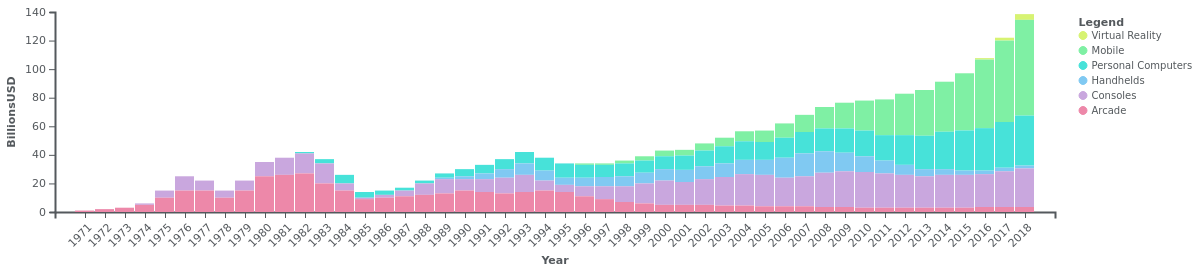
\includegraphics[width=\linewidth]{immagini/valore_commerciale_giochi_globale.png}
	\caption{Ricavi globali dell'industria dei videogiochi dal 1971 al 2018 (non adeguati all'inflazione). Fonte: wikipedia.org}
	\label{fig:valore_commerciale_giochi_globale}
\end{figure}

Per poter far conoscere alle nuove generazioni i videogiochi che hanno fatto la storia e dare la possibilità di poter giocare ancora a macchine che ormai hanno cessato di funzionare per motivi di obsolescenza verranno sfruttati il continuo aumentare della velocità delle connessioni di rete e due tecnologie entrate a far parte della quotidanietà, lo streaming e il cloud computing, rendendo possibile un nuovo modello di consumo: il cloud gaming.

Si propone la creazione di una piattaforma di cloud gaming, che permette lo streaming audio-video direttamente e su richiesta dei videogiochi, da un server remoto, ad un client (computer, console, telefono, tv). Il gioco è archiviato, eseguito, e renderizzato su un server remoto; l'input (tastiera, joystick) viene inviato dal client al server e lì processato. In questo modo si può accedere ai giochi indipendentemente dal sistema operativo e dalle capacità hardware del client utilizzato. Inoltre il cloud gaming permette di iniziare a giocare immediatamente poiché il gioco è già installato sul server offrendo agli utenti una grande semplicità di accesso. Infine la piattaforma, indirettamente, garantisce la gestione dei diritti digitali (DRM) per gli editori.

Verrà ampliato il software MAME (rilasciato sotto licenza GNU-GPL) che è in grado di emulare oltre 7.000 giochi arcade, di modo che possa fungere da server di cloud gaming e comunicare con un front-end HTML, rimanendo sempre indipendente dal sistema operativo, così da rendere più agevole l’installazione di uno stand per il retrogaming.

La tesi è così strutturata: nel Capitolo 1 viene introdotto il cloud gaming e fatta una panoramica dei servizi presenti sul mercato; si descrivono le tecnologie utilizzate nel Capitolo 2, mentre nel Capitolo 3 viene presentata l'architettura del sistema. All’interno del Capitolo 4 vengono illustrati i risultati ottenuti. Nell'ultimo capitolo sono riportate le conclusioni finali e una lista di possibili sviluppi futuri.